\section{Electronic Mail}
Electronic Mail \citep[Chapter 11]{redhatemail} is a communication service which has been used since 1971 \citep{wikiemail} when the first network email with the text ``QWERTYUIOP'' was sent through ARPAnet (Advanced Research Projects Agency Network, the first network which implements the TCP/IP protocol) with the experimental protocol CYPNET. Nowadays, the messages are delivered by using a client/server architecture. In this way, an email is created by using a client-side mail program. Then, this software sends the message to a server, which will redirect to the recipient's mail server. From it, the email is going to be provided to the addressee.

In order to make all this process possible, an Internet standard, that extends the format of email messages, and a wide range of network protocols exist for allowing different machines (often they execute distinct operative systems and make use of different mail programs) to share emails. In this section, we are going to study this standard, these protocols and the API which is going to be used for reading, sending emails and accessing to the user's email data. First of all, we are going to explain the MIME standard (see Section \ref{ssect:mime}) which specifies the format of email message. Then we are going to explain the main email management protocols, both electronic mail transmission protocol (such as Simple Mail Transfer Protocol, which is explained in Section \ref{ssect:smtp}) and message access protocol (such as Internet Message Access Protocol and Post Office Protocol, which are studied in Sections \ref{ssect:imap} and \ref{ssect:pop}, respectively). 

In spite of being a mail server-independent solution, as we will see, we are going to find security issues which are going to hinder our user's email data access. These trials come from the automatic server access. For this reason, Gmail API is going to be introduced (see Section \ref{ssect:gmailapi}) and, finally, the assessment of the advantages and disadvantages of making use of the email protocols or the Gmail API is discussed (see Section \ref{ssect:protvsapi}).

\subsection{MIME} \label{ssect:mime}
To be able to create messages and read the body of the emails, it is essential to understand what the MIME standard consists of. Hence, in this section we are going to give a general idea about this.

MIME, whose acronym stands for Multipurpose Internet Mail Extensions \citep{wikimime}, is an Internet standard for the exchange of several file types (text, audio, video, etc.) which provides support to text with characters other than ASCII, non-text attachments, body messages with numerous parts (known as multi-part messages) and headers information with characters other than ASCII. It is defined in a series of request for comments (RFC): RFC 2045 \citep{rfc2045}, RFC 2046 \citep{rfc2046}, RFC 2047 \citep{rfc2047}, RFC 2049 \citep{rfc2049}, RFC 2077 \citep{rfc2077}, RFC 4288 \citep{rfc4288} and RFC 4289 \citep{rfc4289}.

Virtually all e-mails written by people on the Internet and a considerable proportion of these automatically generated messages are transmitted in MIME format via SMTP (see Section \ref{ssect:smtp}). Internet e-mail messages are so closely associated with SMTP and MIME that they are usually called SMTP/MIME messages.

The content types defined by the MIME standard are of great importance also outside the context of e-mails. Examples of this are some network protocols such as HTTP from the Web. HTTP requires data to be transmitted in an e-mail-type message context although the data may not be an e-mail itself.

Nowadays, no e-mail program or Internet browser can be considered complete if it does not accept MIME in its various facets (text and file formats). 

In this section we will learn how the MIME type nomenclature is (see Section \ref{sssect:MIMEtype}), which is necessary for being able to exchange a several file types. Then, we will illustrate the MIME structure of an email, consisting of MIME headers (see Section \ref{sssect:MIMEheaders}) and, finally, two common MIME message encoding (base64 and quoted-printable) are explained (see Sections \ref{sssect:base64} and \ref{sssect:quot-p}, respectively).

\subsubsection{Type Nomenclature}\label{sssect:MIMEtype}

Each data type has a different name in MIME. These names follow the format: type/subtype (both type and subtype are strings), in such a way that the first denotes the general data category and the second the specific type of that information. The values the type can take are:

\begin{itemize}
	\item\textit{text}: means that the content is simple text. Subtypes like \textit{html}, \textit{xml} and \textit{plain} can follow this type.
	\item\textit{multipart}: indicates that the message has numerous parts with independent data. Subtypes like \textit{form-data} and \textit{digest} can follow this type.
	\item\textit{message}: it is used to encapsulate an existing message, for example when we want to reply a email and add the previous message. Subtypes like \textit{partial} and \textit{rfc822} can follow this type.
	\item\textit{image}: means that the content is an image. Subtypes like \textit{png}, \textit{jpeg} and \textit{gif} can follow this type.
	\item\textit{audio}: indicates that the content is an audio. Subtypes like \textit{mp3} and \textit{32kadpcm} can follow this type.
	\item\textit{video}: denotes that the content is an video. Subtypes like \textit{mpeg} and \textit{avi} can follow this type.
	\item\textit{application}: it is used for application data that could be binary. Subtypes like \textit{json} and \textit{pdf} can follow this type.
	\item\textit{font}: means that the content is a file which defines a font format. Subtypes like \textit{woff} and \textit{ttf} can follow this type.
\end{itemize}

\subsubsection{MIME headers} \label{sssect:MIMEheaders}

MIME has several headers which appear in all emails sent with this standard. The most important of them are the following:

\begin{itemize}
	\item\textit{Content-Type}: the value of this header is the type and subtype of the message with the same structure that we have explained before. For example, if we have the header \textit{Content-Type: text/plain}, it means that the message is a plain text. By using the type \textit{multipart} make the creation of messages with parts and subparts organized in a tree structure (in which leaf nodes can belong to any type and the rest of them can belong to any multipart subtype variety) possible \citep[Section 7.2]{rfc1341}. A feasible composition of a message with a part with plain text and other non-text parts could be constructed by using \textit{multipart/mixed} as the root node like in Figure \ref{fig:content-type}. Indeed, in the example of Figure \ref{fig:content-type}, we can observe the use of \textit{multipart/alternative} for a message which contains the body both in plain text and in html text. Other different emails constructions are possible (like forwarding with the original message attached by using \textit{multipart/mixed} with a \textit{text/plain} part and a \textit{message/rfc822} part) thanks to the tree structure of the \textit{Content-type} header.
	
	Another important detail, that we can observe in the example in figure \ref{fig:content-type}, is the fact that each node of the tree structure of the emails is visited and showed following the pre-order traversal.
	
	\begin{figure}[t]
		\centering%
		\includegraphics[width = 1.2\textwidth]{Imagenes/Bitmap/tree-content-type.png}%
		\caption{MIME types tree structure of an email example}%
		\label{fig:content-type}
	\end{figure}
	\item\textit{Content-Disposition}: this header is used to indicate the presentation style of the part of the message. There are two ways to show the part: \textit{inline} content-disposition (which means that the content must be displayed at the same time as the message) and \textit{attachment} content-disposition (the part is not displayed at the same time as the message and it requires some form or action from the user to see it). Furthermore, this header also provides several fields for specifying other type of information about the content, such as the name of the file and the creation or modification date. The following example is taken from RFC 2183 \citep{rfc2183} and, as we will explain after the example, it does not match with the syntax of this same header in the example that we can see in the last part of the example message of figure \ref{fig:content-type}:
	\begin{lstlisting}
	Content-Disposition: attachment; filename=genome.jpeg;
	modification-date="Wed, 12 Feb 1997 16:29:51 -0500";
	\end{lstlisting}
	As we have said, this syntax is different from the used in the email example of Figure \ref{fig:content-type}. This results from the fact that, in HTTP, the header we find in that figure (\textit{Content-Disposition: attachment}) is usually used for instructing the client to show the response body as a downloadable file. As we can observe, it has a \textit{filename} field which is used for establishing the default file name when the user is going to download it.
	
	\item\textit{Content-Transfer-Encoding}: when we want to send some files in a message, sometimes they are represented as 8-bit character or binary data, which are not allowed in some protocols. On this account, it is necessary to have a standard that indicates how we should re-encoding such data into a 7-bit short-line format. The Content-Transfer-Encoding header \citep[Section 5]{rfc1341} will tell the client which transformation has been used for being able to transport that data. Therefore and for lack of a previous standard which states a single Content-Transfer-Encoding mechanism, the possible values, which specify the type of encoding are: \textit{'base64'} (see Section \ref{sssect:base64}), \textit{'quoted-printable'} (see Section \ref{sssect:quot-p}), \textit{'8bit'}, \textit{'7bit'}, \textit{'binary'} and \textit{'x-token'}. All these values are not case sensitive. If this header does not exist, we can assume that the value of this header is \textit{'7bit'}, which means that the body of the message is already in a seven-bit mail-ready representation, in other words, all the body of the message is represented as short lines of US-ASCII data. Despite the \textit{'8bit'}, \textit{'7bit'} and \textit{'binary'} indicate that the content has not been transformed, they are useful for knowing the kind of encoding that the data has. This header will generally be omitted when the Content-Type has the \textit{multipart} or \textit{'message'} type (as it happens in the message example of Figure \ref{fig:content-type}), because it also admits the last three types we have mentioned.
	
	It is common to add another header (as we can see in Figure \ref{fig:content-type}) called \textit{charset}, which value represents the original encoding of data so the client is able to decode it.
\end{itemize}

\subsubsection{Base64} \label{sssect:base64}
As we have studied when we learnt how the MIME headers (see Section \ref{sssect:MIMEheaders}) are, we can find email whose content encoding is base64. Base64 \citep{wikibase64, rfc4648} is a group of reversible binary-to-text encoding schemes which represent binary data as a sequence of ASCII printable characters. It makes use of a radix-64 to translate each character, because 64 is the higher power of two than can be represented using only printable ASCII characters. Indeed all the Base64 variants (like base64url) utilise the characters range A-Z, a-z and 0-9 in that order for the first 62 digits, but the chosen symbol for the last two digits are very different between them. In particular, the MIME (see Section \ref{ssect:mime}) specification, established in RFC 2045 \citep{rfc2045}, describes base64 based on  Privacy-enhanced Electronic Mail (PEM) protocol \citep{wikipem, rfc7468}, which means that the last two characters are '+' and '/' and the symbol '=' is used for output padding suffix. In the same way, MIME does not stablish a fixed size for the base64 encoded lines, by contrast it specifies a maximum size of 76 characters.

If we try to apply standard base64 in a URL encoder, it will translate the characters '+' and '/' to its hexadecimal representation ('+' = '\%2B' y '/' = '\%2F'). This will cause a conflict in heterogeneous systems or if we use it in data base storage, because of the character '\%' produced by the encoder (it is a special symbol of ANSI SQL). This is why modified Base64 for URL variants exists (such as base64url in \cite{rfc4648}), where the '=' character has no usefulness and the '+' and '/' symbols are replaced by '-' and '\_' respectively. Besides it has no impact on the size of encoded lines.

\subsubsection{Quoted-printable} \label{sssect:quot-p}
Other reversible binary-to-text encoding that could be used in the content of a MIME message is the quoted-printable encoding \citep{wikiquotprint, rfc1521}. Making use of printable characters (such as alphanumeric and '=') proved capable of transmitting 8 bit data over a 7 bit protocol. Unlike base64, if the original message is mostly composed of ASCII characters, the encoded text is readable and compact.

Each byte could be represented via two hexadecimal character. On this basis, the '=' symbol followed by two hexadecimal digits are enough to encode all the characters except the printable ASCII ones and the end of line. For example, if we want to represent the 12th ASCII character we can encode it as '=0C' or if the equality symbol (whose decimal value is 61) is in our original message, it could be encoded as '=3D' (note that despite being a printable ascii character it must be encoded as it is a special character in this encoding). This is how quoted-printable encodes the different characters.

In respect of the maximum line size, as it happens with the MIME specification of the base64 (see Section \ref{sssect:base64}), it is 76 characters each encoded line. To achieve this goal and still be able to decode the text getting the original message, quoted-printable adds \textit{soft line breaks} at the end of the line consisting of the '=' symbol and it does not modify the encoded text.

\subsection{Simple Mail Transfer Protocol} \label{ssect:smtp}

Simple Mail Transfer Protocol (also known as SMTP) is a network connection-oriented communication protocol used for the exchange of e-mail messages. It was originally defined in \cite{rfc821} (for the transfer) and in \cite{rfc822} (for the message). It is currently defined in \cite{rfc5321} and \cite{rfc5322}. However, this protocol has some limitations when it comes to receiving messages on the destination server. For this reason, this task is intended for other protocols such as the Internet Message Access Protocol (see Section \ref{ssect:imap}) or the Post Office Protocol (refer to Section \ref{ssect:pop}), and SMTP is used specifically to send messages.

Making use of SMTP, an email is ``pushed'' from one mail server to another (next-hop mail server) until it reaches its destination. The message is not routed according to the message recipients specified during the client's connection to the SMTP server, but from the destination mail server. Thanks to the fact that this protocol has a feature to initiate mail queue processing, an intermittently connected mail server can extract messages from another remote server when necessary.

\subsection{Post Office Protocol} \label{ssect:pop}

Post Office Protocol (also known as POP) is an application protocol (in OSI Model) for obtaining e-mails stored in a remote Internet server called POP server. It was originally defined in \cite{rfc918} (it was POP version 1, also known as POP1). Current POP version (POP3, in general when we talk about POP we refer to this version) is detailed in \cite{rfc1939}.

POP was designed for receiving emails. Using POP, users with intermittent or very slow Internet connections (such as modem connections) can download their email while online and check it later even when offline. The general operation is: a client using POP3 connects, gets all messages, stores them on the user's computer as new messages, deletes them from the server, and finally disconnects. However some mail clients include the option to leave messages on the server. They use the order UIDL (Unique IDentification Listing) which, unlike most POP3 commands, does not identify messages depending on their mail server ordinal number. This results from the fact that the mail server ordinal number creates problems when a client tries to leave messages on the server, since messages with numbers change from one connection to the server to another. Accordingly, server which makes use of UIDL, assigns a unique and permanent character string to each message. Thus, when a POP3-compatible mail client connects to the server, it uses the UIDL command to map the message identifier. This way the client can use that mapping to determine which messages to download and which to save at the time of downloading.

Like other old Internet protocols, POP3 used a signature mechanism without encryption. The transmission of POP3 passwords in plain text still occurs. Nowadays POP3 has various authentication methods that offer a diverse range of levels of protection against illegal access to users' mailboxes.

The advantage over other protocols is that between server-client you do not have to send so many commands for communication between them. The POP protocol also works properly if you do not use a constant connection to the Internet or to the network that contains the mail server.

\subsection{Internet Message Access Protocol} \label{ssect:imap}

Internet Message Access Protocol (also known as IMAP) is an application protocol, designed as an alternative to Post Office Protocol (se Section \ref{ssect:pop}) in 1986, which allows the access to stored messages in an Internet server. As with the Post Office Protocol, with IMAP you can access your e-mail from any computer with an Internet connection. The current version of IMAP (IMAP version 4 review 1 or IMAP4rev1) is defined in \cite{rfc3501}.

In contrast to Post Office Protocol, IMAP allows multiple clients to manage the same mailbox. This fact results from the main differences between these two protocols: IMAP does not remove email from server until the client specifically requests it (as POP removes them by default, it is impossible to accessing them from another device which has not the downloaded messages) and it does not download the messages to the user's computer (clients may optionally store a local copy of them). This last property gives raise to several advantages with regard to Post Office Protocol: the immediate notification of the arrival of a mail (due to it works in permanent connection mode) while POP checks if there are new e-mails every few minutes (which causes an appreciable rise in traffic and in the time the user has to wait to send a request to the server, because it is necessary to complete the download of all new messages first), it is possible to create shared folders with other users (it depends on the mail server), the e-mails do not take up memory in the user's local device while POP downloads them regardless of whether they are going to be read or not (effectively IMAP has to download a message when it is going to be read, but they are temporary files and only the e-mail headers are downloaded to manage the mailbox) and it allows the user to manage folders, templates and drafts in server in addition to be able to search a mail from keywords.

\subsection{Gmail API}\label{ssect:gmailapi}
Gmail is a free email service developed by the company Google. Users can access Gmail on the web itself and through third-party programs that synchronize email content via POP or IMAP protocols. It also has a mobile application to manage the user's email. Gmail began as a limited beta version on April 1, 2004 and completed its testing phase on July 7, 2009. As stated in \cite{gmailbbc}: ``Gmail is the world's most popular email service with 1.4 billion users''.

As we will see in Section \ref{ssect:protvsapi}, due to the automatic server access, directly using the communication protocol for electronic mail transmission (SMTP) and for retrieving email messages from a mail server (POP or IMAP) will cause us security problems in accessing the user's email data. For this reason, we are going to make use of Gmail API. In this section we are going to study it. Thus in Section \ref{sssect:oauth}, we are going to study the necessary protocol for accessing the Gmail API and consequently for being able to get into the user's email data. Further on, we will require a resource (like a programming object) we can work with and represent all the Gmail structure (see Section \ref{sssect:usersres}). Once we count on this general resource, we have the necessary tools to be able to understand and handle the internal architecture of the Gmail API and the different means it provides in order to achieve our goal. Therefore, in Sections \ref{sssect:labres}, \ref{sssect:msgres}, \ref{sssect:threads} and \ref{sssect:drafts} we are going to delve into the essential resources for our purpose: labels, messages, threads and drafts, respectively.

Finally, as this API is not the only means of accessing the user's mail data (we have studied other ways in previous sections), we will end with a brief description about the API usage limits (in Section \ref{sssect:apilimits}) to assess its use with respect to other methods of email access.

\subsubsection{OAuth 2.0 Protocol}\label{sssect:oauth}
Open Authorization or OAuth \citep{oauth} is an open standard which allows simple authorization flows for web services or applications. It is a protocol defined in \cite{rfc6749} which allows the site's users to share their information with another site without providing their full identity. This mechanism is used by companies like Google, Facebook, Twitter and Microsoft to allow users to share information about their accounts with third-party applications or websites

Gmail API, as it also happens in the case of other Google APIs, uses OAuth 2.0 protocol \citep{oauthforgoogle} to handle authentication and authorization. It will provide us a secure and trusted login system to access to the user's Gmail data.

The basic working process of OAuth 2.0 protocol can bee seen in Figure \ref{fig:oauth}. As we can observe, at first our application carries out a request in which it sends a token. This token includes, among other things, a credential, which helps Google Servers  to identify the application, and a list of OAuth 2.0 Scopes \citep{oauth-scopes-google}, which are a ``mechanism  in OAuth 2.0 to limit an application's access to a user's account. An application can request one or more scopes. This information is then presented to the user in a consent screen, and the access token issued to the application will be limited to the scopes granted'' \citep{oauth-scopes}. We will use the Gmail API OAuth 2.0 Scope which allows us to read, compose, send, and delete emails.

Once the user has logged in the Gmail account (authentication) and accepted all the necessary permissions that our application needs (authorization), our process receives an authorization code which is going to be exchanged for an access token \citep{oauth-exchange}. Then, we will be in possession of the OAuth 2.0 credentials for the user \citep{oauth2.credentials} which we are going to use for accessing the user's Gmail account.

\begin{figure}[h]
	\centering%
	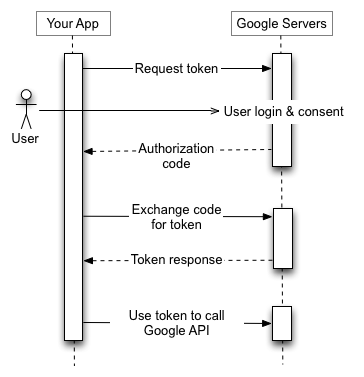
\includegraphics[width = 0.5\textwidth]{Imagenes/Bitmap/webflow.png}%
	\caption{OAuth 2.0 for Web Server Applications and Installed Applications.}%
	Image extracted from \cite{oauthforgoogle}
	\label{fig:oauth}
\end{figure}

\subsubsection{Users resource}\label{sssect:usersres}
At this point, with the OAuth 2.0 credentials, we are able to call the Gmail API. For this purpose, it is necessary to construct a resource \citep[/v1/reference]{gmailAPI} for interacting with the API. As we will see later, this resource will lead us to manage emails, drafts, threads and everything we will like to do with the user's Gmail data.

By using the OAuth 2.0 credentials, we are able to get in contact with the Google Servers and request for what is known as users resource \citep[/v1/reference/users]{gmailAPI}, which holds all the necessary resources for our task, such as labels (see Section \ref{sssect:labres}), messages (see Section \ref{sssect:msgres}), threads (see Section \ref{sssect:threads}) and drafts (see Section \ref{sssect:drafts}). In practice, the users resource has instance methods which get in contact with Google Servers and return these other Gmail API resources that we are going to need (the methods' names are \textit{labels()}, \textit{messages()}, \textit{threads()} and \textit{drafts()}, respectively). Now, in next sections, we are going to explain all the resources we can create with the user resource.

\subsubsection{Labels resource}\label{sssect:labres}
As we have seen in the explanation of the users resource (Section \ref{sssect:usersres}), we can obtain the labels resource \citep[/v1/reference/users/labels]{gmailAPI} by invoking \textit{labels()} instance method of our users resource. It manages the entire set of our email labels, which  categorize messages and threads within the user's mailbox.

Labels resource is an object which allows us to access to the different email labels of the user, such as \textit{INBOX}, \textit{UNREAD} and \textit{SENT}. With the labels resource methods, we can obtain each of these ``user's labels'' which have a dictionary structure and their representation is what we can observe hereunder:

\begin{python}
	{
		'id' : string, # The immutable identifier of the label
		'name' : string, # The display name
		# The visibility of messages in the Gmail web interface
		'messageListVisibility' : string,
		'labelListVisibility' : string, # The visibility of label
		'type' : string, # The owner type of the label ('system' or 'user')
		'messagesTotal' : integer, # Total number of messages with the label
		'messagesUnread' : integer, # Number of unread messages with the label
		'threadsTotal' : integer, # Total number of threads with the label
		'threadsUnread' : integer, # Number of unread threads with the label
		'color' : {
			# Text color of the label, represented as hex string
			'textColor' : string,
			# Background color represented as hex string #RRGGBB
			'backgroundColor' : string 
		}
	}
\end{python}

The important fields we are going to need are the \textit{name}, the \textit{type} and the number of total messages and threads with the label (which are \textit{messagesTotal} and \textit{threadsTotal} fields, respectively). Labels with \textit{system} type, such as \textit{INBOX}, \textit{SENT}, \textit{DRAFTS} and \textit{UNREAD}, are internally created and cannot be added, modified or deleted.

\subsubsection{Messages resource}\label{sssect:msgres}
In most of the operations we are going to execute, the correct management of messages will be essential. Therefore, knowing how the emails are represented in Gmail API and how to use them is imperative to understand how to work with this API. For this reason, in this section we are going to delve into the messages resource \citep[/v1/reference/users/messages]{gmailAPI} of the Gmail API. As we saw in Section \ref{ssect:userres}, we can access to this resource by invoking the \textit{messages()} instance method when we have a users resource.

As with the labels resource, the messages resource manages the set of all messages of the user's email. With the messages resource methods, we can obtain each of these ``user's messages'' which, regardless of which programming language is used, have a dictionary structure and their representation is what we can see down below:

\begin{python}
	{
		'id' : string,
		'threadId' : string,
		'labelIds' : [ string ],
		'snippet' : string,
		'historyId' : unsigned long,
		'internalDate' : long,
		'payload' : {
			'partId' : string,
			'mimeType' : string,
			'filename' : string,
			'headers' : [
			{
				'name' : string,
				'value' : string
			}
			],
			'body' : {
				'attachmentId' : string,
				'size' : integer,
				'data' : bytes
			},
			'parts' : [ (MessagePart) ]
		},
		'sizeEstimate' : integer,
		'raw' : bytes
	}
\end{python}

The more important keys of this data structure for this work are:
\begin{itemize}
	\item\textit{id}: an immutable string which identifies the message.
	\item\textit{threadId}: we will explain the thread resource in Section \ref{sssect:threads} and we will see that a thread is composed of different messages that share common characteristics. The value of this field is a string which represent the identifier of the thread the message belongs to.
	\item\textit{labelIds}: a list of the identifiers of labels (see Section \ref{sssect:labres}) applied to the message.
	\item\textit{payload}: as we can see in the resource representation above, it has a dictionary data structure. The \textit{payload} field is the parsed email structure in the message parts. The more important keys of the \textit{payload} field are:
	\begin{itemize}
		\item\textit{mimeType}: the MIME type (see the explanation of \textit{Content-Type} header in Section \ref{sssect:MIMEheaders}) of the message part.
		\item\textit{headers}: a list of headers. It contains the standard RFC 2822 \citep{rfc2822} email headers such as \textit{To}, \textit{From}, \textit{Subject} and \textit{Date}. Each header has a \textit{name} field, which is the name of the header (for example \textit{From}), and a \textit{value} field, which is the value of the header (following the same example as with the \textit{name} field: \textit{example@gmail.com} could be the value).
		\item\textit{parts}: a list which contains the different MIME message child parts (we have gone into it in depth in the Section \ref{ssect:mime}).
		\item\textit{body}: a dictionary structure which contains the body data of this part (see Section \ref{ssect:mime}) in case it does not contain MIME message parts (otherwise it will be empty). This structure should not be confused with an attached file. Each MIME part contains a body property regardless of MIME type of the part.
	\end{itemize}
	\item\textit{raw}: the entire email message in an RFC 2822 \citep{rfc2822} formatted and base64url (see Section \ref{sssect:base64}) encoded string.
\end{itemize}

\subsubsection{Threads resource}\label{sssect:threads}
When we access to our inbox, we are actually seeing the inbox threads instead of the messages resource. Every message, even if it is an only email without a reply, is enclosed in a thread resource \citep[/v1/reference/users/threads]{gmailAPI} which is essentially a list, perhaps unitary, of messages resources. In fact, as we can observe in the following resource representation, each thread (which can be obtained thanks to the threads resource due to it manages the entire set of threads of a user's email), in its dictionary structure, has a list of messages resources:

\begin{python}
	{
		'id' : string, # The identifier of the thread
		'snippet' : string, # A short part of the text
		'historyId' : unsigned long,
		'messages' : [ users.messages resource ]
	}
\end{python}

\subsubsection{Drafts resource}\label{sssect:drafts}
The last Gmail API resource we will study is the most easy to understand after knowing all the structures related with emails that we have explained in the above sections: the drafts resource \citep[/v1/reference/users/drafts]{gmailAPI}. Its representation is very simple:

\begin{python}
	{
		'id' : string # The immutable identifier of the draft
		'message' : users.messages resource
	}
\end{python}

As we can observe, a draft is virtually a messages resource with an identifier. Indeed, in order to create a new draft with the \textit{DRAFT} label we must create a MIME message (see Section \ref{ssect:mime}) as we have to do when we want to send a new email by using the \textit{send} messages resource method.

\subsubsection{API Usage Limits} \label{sssect:apilimits}
One factor to be taken into account is the limitations of the Gmail API \citep[/v1/reference/quota]{gmailAPI} which could become a drawback in the application development. It has a limit on the daily usage and on the per-user rate. In order to measure the usage rate, ``quota units'' are defined depending on the method invoked (main methods of each resource are explained in Section \ref{sect:gmailapitech}). In Table \ref{tab:quotaUnits} we can consult the value of some methods in quota units (we have selected the more important methods for our purpose, for the quota units of other methods it is recommended to refer to \cite[/v1/reference/quota]{gmailAPI}).

\begin{table}[h]
	\centering
	\begin{tabular}{|l c r|}
		\hline
		\textbf{Method} & \textbf{Where the method is explained} & \textbf{Quota units} \\
		\hline\hline
		\textit{getProfile} & \ref{ssect:userres} & 1\\ \hline
		\textit{labels.get} & \ref{ssect:labres} & 1\\ \hline
		\textit{messages.get} & \ref{ssect:msgres} & 5\\ \hline
		\textit{messages.list} & \ref{ssect:msgres} & 5\\ \hline
		\textit{messages.send} & \ref{ssect:msgres} & 100\\ \hline
		\textit{threads.get} & \ref{ssect:threads} & 10\\ \hline
		\textit{threads.list} & \ref{ssect:threads} & 10\\ \hline
		\textit{drafts.create} & \citep[/v1/reference/users/drafts]{gmailAPI} & 10\\ \hline
	\end{tabular}
	\caption{Main methods' quota units}
	\label{tab:quotaUnits}
\end{table}

However, both daily usage limit and per-user rate limit are acceptable for the type of software we want to build: 1,000,000,000 quota units per day and 250 quota units per user per second. Therefore there are no constraints (for our purpose) that avoid us to use this API.

\subsection{Advantages and disadvantages of email protocols versus the use of Gmail API} \label{ssect:protvsapi}
Without using the Gmail API, we may be able to access mail accounts by implementing the different email protocols that we have studied. Indeed, this implementation would allow us to access them regardless of the mail server, in other words, we would be able to work with any email account without the need of being a Gmail one. However, when we try to developed an application which is going to access to a user's email account, Google Servers detect it as a non-authorised login and block the authentication process. Then they send to the user a warning titled ``A login attempt has been blocked'' with the following information:

``\textit{Someone just used your password to try to sign in to your account from a non-Google application. Although Google has blocked access, you should find out what happened. Check your account activity and make sure that only you have access to your account.}''

Against this background, it is possible to change the user's security settings for allowing the automatic accessing to the account. However, it is not recommended (due to possible security issues) and creates a sense of insecurity for the user of the application that requires this configuration.

In the other hand we have the Gmail API, which facilitates the access to email's data. Besides, its only disadvantage is to limit the daily usage of this technology by imposing quota units. However, this quota units are enough for achieving our aim. For these reasons, and because of the email accounts that we will study belongs to Gmail, the Gmail API has been chosen as the most suitable way for managing the user's email account.